\documentclass[11pt,letterpaper]{article}
\usepackage[lmargin=1in,rmargin=1in,tmargin=1in,bmargin=1in]{geometry}
\usepackage{../style/homework}
\usepackage{../style/commands}
\setbool{quotetype}{true} % True: Side; False: Under
\setbool{hideans}{true} % Student: True; Instructor: False

% -------------------
% Content
% -------------------
\begin{document}

\homework{9: Due 11/09}{I did not attend his funeral, but I sent a nice letter saying I approved of it.}{Mark Twain} 

% Problem 1
\problem{10} Find the least square regression line for the points: $(1, 1), (1,0), (2,3), (3,4)$. Show all your work. 





\newpage





% Problem 2
\problem{10} Given the following information below, find the least square regression line. Show all your work. 
	\[
	\begin{aligned}
	n&= 11 \\
	\overline{x}&= 3.45, \quad \sigma_x^2&= 7.073 \\
	\overline{y}&= 6.81, \quad \sigma_y^2&= 5.371 \\
	R&= 0.802
	\end{aligned}
	\]





\newpage





% Problem 3
\problem{10} Match each regression coefficient to its corresponding graph. 
	\begin{figure}[!ht]
	\centering
	\begin{minipage}{0.45\textwidth}
	   \centering
	   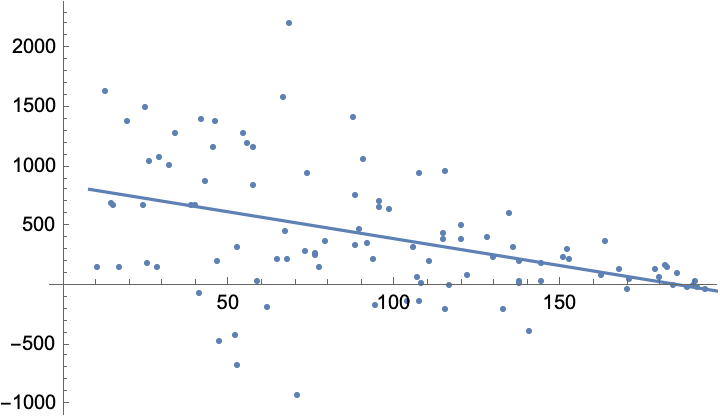
\includegraphics[width=0.9\textwidth]{reg1.png}
	   \caption*{(a)}
	\end{minipage}\hfill
	\begin{minipage}{0.45\textwidth}
	   \centering
	   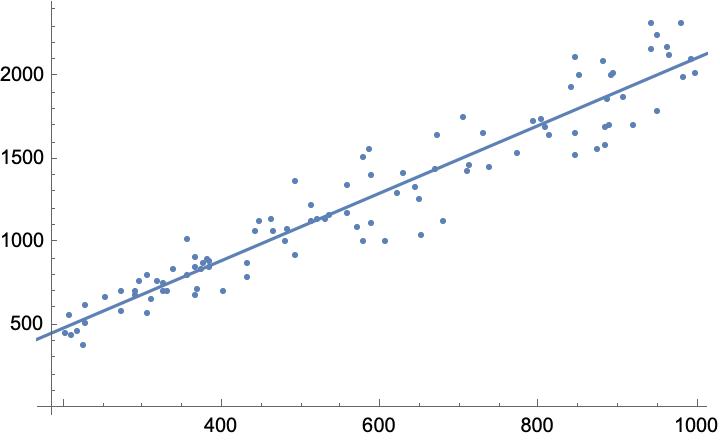
\includegraphics[width=0.9\textwidth]{reg2.png}
	   \caption*{(b)}
	\end{minipage}
	\begin{minipage}{0.45\textwidth}
	   \centering
	   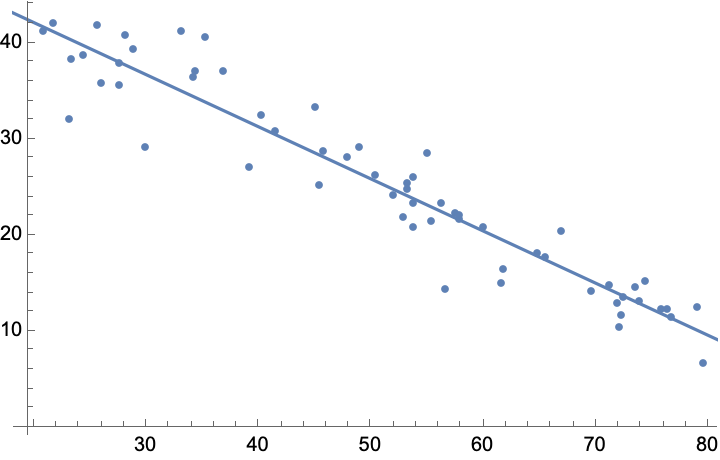
\includegraphics[width=0.9\textwidth]{reg3.png}
	   \caption*{(c)}
	\end{minipage}
	\begin{minipage}{0.45\textwidth}
	   \centering
	   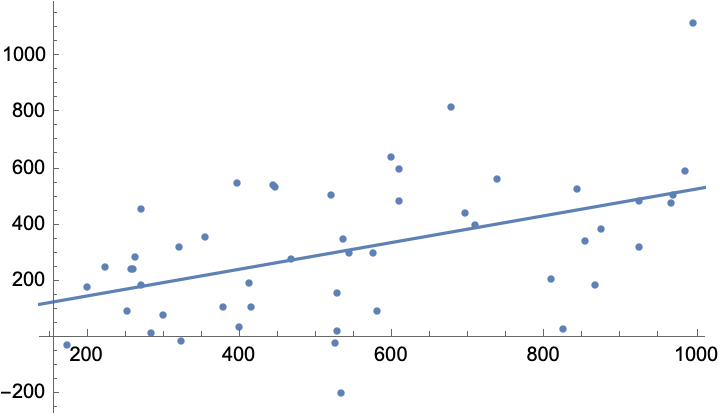
\includegraphics[width=0.9\textwidth]{reg4.png}
	   \caption*{(d)}
	\end{minipage}
	\end{figure}

\begin{enumerate}[(i)]
\item \underline{\hspace{1.5cm}}: $R= -0.9529$
\item \underline{\hspace{1.5cm}}: $R= -0.4354$
\item \underline{\hspace{1.5cm}}: $R= 0.4759$
\item\underline{\hspace{1.5cm}}: $R= 0.9573$
\end{enumerate} 





\newpage





% Problem 4
\problem{10} The lengths (in cm) of twenty snakes are taken 6~months after hatching and 2~years after hatching. The data is given below.
	\[
	\begin{aligned}
	(41.2, 163.6), (18.1, 68.9), (42.3, 151.6), (13.2, 43.9), (45.8, 189.5), \\ 
	(42.7, 180.5), (24.4, 92.8), (49.0, 166.), (24.6, 101.1), (18.9, 77.5), \\
	(16.3, 63.6), (36.3, 142.2), (32.2, 124.3), (36.3, 121.), (24.7, 77.8), \\
	(40.1, 139.7), (22.3, 72.8), (42.4, 182.2), (21.4, 73.), (12.3, 53.1)
	\end{aligned}
	\]
A linear regression for this data was found to be $\widehat{y}= 3.9x - 3.1$ with $R= 0.9381$. 
	\begin{enumerate}[(a)]
	\item Was the linear regression a good fit for the data? Explain.
	\item Find the residual for the data point $(41.2, 163.6)$. Was the model under or over prediction for the length of the snake? Explain.
	\item Given this data and model, predict the length of a snake after 2~years that measures 32.7~cm 6~months after hatching. 
	\item Should this model be used to predict the length of a snake which is 65~cm six months after hatching? Explain. 
	\end{enumerate}





\end{document}